% Uebung Nr. 7 Zeigerdiagramm nach Brinkmeyer
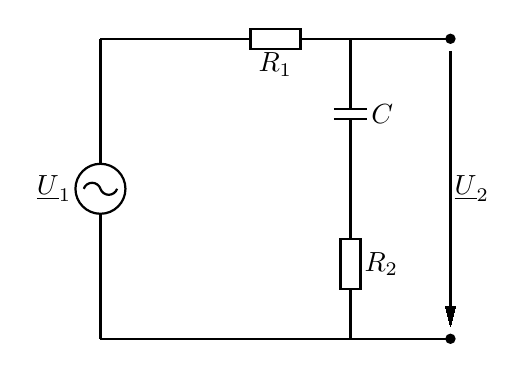
\begin{tikzpicture}[scale=2.54]%
% dpic version 2024.01.01 option -g for TikZ and PGF 1.01
\ifx\dpiclw\undefined\newdimen\dpiclw\fi
\global\def\dpicdraw{\draw[line width=\dpiclw]}
\global\def\dpicstop{;}
\dpiclw=0.8bp
\dpiclw=0.8bp
\dpicdraw (0,0)
 --(0,-0.625)\dpicstop
\dpicdraw (0,-0.75) circle (0.049213in)\dpicstop
\dpicdraw (-0,-0.75)
 ..controls (-0.005978,-0.732065) and (-0.022762,-0.719968)
 ..(-0.041667,-0.719968)
 ..controls (-0.060571,-0.719968) and (-0.077355,-0.732065)
 ..(-0.083333,-0.75)\dpicstop
\dpicdraw (0,-0.75)
 ..controls (0.005978,-0.767935) and (0.022762,-0.780032)
 ..(0.041667,-0.780032)
 ..controls (0.060571,-0.780032) and (0.077355,-0.767935)
 ..(0.083333,-0.75)\dpicstop
\dpicdraw (0,-0.875)
 --(0,-1.5)\dpicstop
\draw (-0.125,-0.75) node[left=-2bp]{$ \underline{U}_1$};
\dpicdraw (0,0)
 --(0.5,0)\dpicstop
\dpicdraw (0.5,0)
 --(0.75,0)\dpicstop
\dpicdraw (1,0)
 --(1,0.05)
 --(0.75,0.05)
 --(0.75,-0.05)
 --(1,-0.05)
 --(1,0)\dpicstop
\dpicdraw (1,0)
 --(1.25,0)\dpicstop
\draw (0.875,-0.05) node[below=-2bp]{$ R_1$};
\dpicdraw (1.25,0)
 --(1.25,-0.35)\dpicstop
\dpicdraw (1.166667,-0.35)
 --(1.333333,-0.35)\dpicstop
\dpicdraw (1.166667,-0.4)
 --(1.333333,-0.4)\dpicstop
\dpicdraw (1.25,-0.4)
 --(1.25,-0.75)\dpicstop
\draw (1.333333,-0.375) node[right=-2bp]{$ C$};
\dpicdraw (1.25,-0.75)
 --(1.25,-1)\dpicstop
\dpicdraw (1.25,-1.25)
 --(1.3,-1.25)
 --(1.3,-1)
 --(1.2,-1)
 --(1.2,-1.25)
 --(1.25,-1.25)\dpicstop
\dpicdraw (1.25,-1.25)
 --(1.25,-1.5)\dpicstop
\draw (1.3,-1.125) node[right=-2bp]{$ R_2$};
\dpicdraw (1.25,0)
 --(1.75,0)\dpicstop
\dpicdraw[fill=black](1.75,0) circle (0.007874in)\dpicstop
\dpicdraw[fill=black](1.75,-1.5) circle (0.007874in)\dpicstop
\filldraw[line width=0bp](1.725,-1.34)
 --(1.75,-1.44)
 --(1.775,-1.34) --cycle\dpicstop
\dpicdraw (1.75,-0.06)
 --(1.75,-1.417094)\dpicstop
\draw (1.75,-0.75) node[right=-2bp]{$ \underline{U}_2$};
\dpicdraw (1.75,-1.5)
 --(0,-1.5)\dpicstop
\end{tikzpicture}%
